\subsection{Missing Value and the Reason to Take Mean}

As we can see, (\expandafter{\romannumeral1}) the attributes recorded by each weather station are quite different, (\expandafter{\romannumeral2}) there are lots of missing values for each day. However, since the time sequence is significantly importance for our study, we can not afford to remove any single row in the data. It is also not feasible to substitute the missing values because of sparsity of the dataset. Instead, since we have records from approximately 100 stations each day, we can take mean of each scalar attribute (temperature, precipitation, etc.), and take weighted mean vector of each vector attribute (attributes related to wind). By doing so we have a row that contains all the attributes for each date, and remove the attributes that still have missing values.

As we can see, the attributes recorded by each weather station are quite different, and there are lots of missing values for each day. However, since the time sequence is significantly importance for our study, we can not afford to remove any single row in the data. It is also not feasible to substitute the missing values because of the sparsity of the dataset. The first way is performing clustering based on the location of stations, substitute missing values with the mean of variables within each cluster. As shown in Figure \ref{clust}, we have the largest average silhouette width when k = 2. The map plot on the right hand side of Figure \ref{clust} shows the clustering result, basically the stations are separated into two clusters, west and east, with downtown Seattle as the boundary in the middle. However, with this method we may create missing values since some of the variables are only recorded by stations in one cluster. Also it is hard to tell the relationship between clusters and the way to combine variables is harder. Therefore, we decided not to use clustering for substituting missing values.
 
Instead, since we have records from approximately 100 stations each day, we can group by date and take mean of each scalar attribute (temperature, precipitation, etc.) directly, and take weighted mean vector of each vector attribute (attributes related to wind). By doing so we have a row that contains all the attributes for each date, and remove the attributes that still have missing values.

\begin{figure}[h]
\centering
\begin{minipage}[t]{0.48\textwidth}
\centering
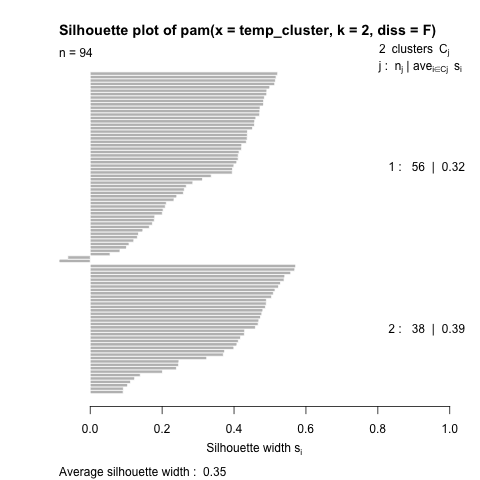
\includegraphics[width=6cm]{silhouette.png}
\end{minipage}
\begin{minipage}[t]{0.48\textwidth}
\centering
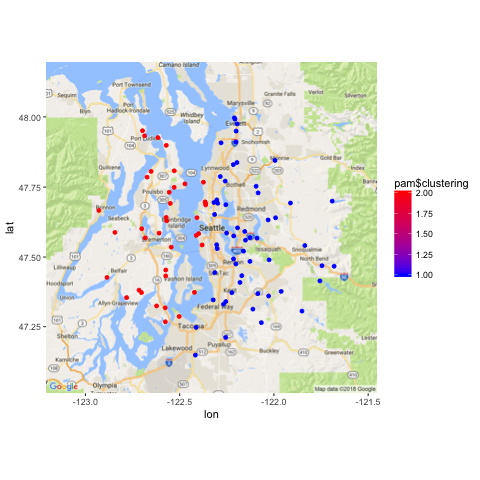
\includegraphics[width=6cm]{clustermap.png}
\end{minipage}
\caption{Clustering Results}
\label{clust}
\end{figure}